\documentclass[11pt,]{article}

\usepackage{lmodern}

\usepackage{amssymb,amsmath}
\usepackage{ifxetex,ifluatex}
\usepackage{fixltx2e} % provides \textsubscript
\ifnum 0\ifxetex 1\fi\ifluatex 1\fi=0 % if pdftex
  \usepackage[T1]{fontenc}
  \usepackage[utf8]{inputenc}
\else % if luatex or xelatex
  \ifxetex
    \usepackage{mathspec}
    \usepackage{xltxtra, xunicode}
  \else
    \usepackage{fontspec}
  \fi
  \defaultfontfeatures{Mapping=tex-text, Scale=MatchLowercase}
  \newcommand{\euro}{€}
\fi

% use upquote if available, for straight quotes in verbatim environments
\IfFileExists{upquote.sty}{\usepackage{upquote}}{}
% use microtype if available
\IfFileExists{microtype.sty}{%
\usepackage{microtype}
\UseMicrotypeSet[protrusion]{basicmath} % disable protrusion for tt fonts
}{}
\usepackage[top=0.5in, bottom=.4in, left = 1in, right=1in, includeheadfoot]{geometry}
\ifxetex
  \usepackage[setpagesize=false, % page size defined by xetex
              unicode=false, % unicode breaks when used with xetex
              xetex]{hyperref}
\else
  \usepackage[unicode=true]{hyperref}
\fi
\hypersetup{breaklinks=true,
            bookmarks=true,
            pdfauthor={Ph. D. Pablo Eduardo Caicedo R.},
            pdftitle={Actividad 001: Fundamentos de Python y RMarkdown},
            colorlinks=true,
            citecolor=blue,
            urlcolor=blue,
            linkcolor=magenta,
            pdfborder={0 0 0}}
\urlstyle{same}  % don't use monospace font for urls
\usepackage{longtable,booktabs}
\usepackage{graphicx}
\makeatletter
\def\maxwidth{\ifdim\Gin@nat@width>\linewidth\linewidth\else\Gin@nat@width\fi}
\def\maxheight{\ifdim\Gin@nat@height>\textheight\textheight\else\Gin@nat@height\fi}
\makeatother
% Scale images if necessary, so that they will not overflow the page
% margins by default, and it is still possible to overwrite the defaults
% using explicit options in \includegraphics[width, height, ...]{}
\setkeys{Gin}{width=\maxwidth,height=\maxheight,keepaspectratio}
% \setlength{\parindent}{0pt}
\setlength{\parskip}{6pt plus 2pt minus 1pt}
\setlength{\emergencystretch}{3em}  % prevent overfull lines
\setcounter{secnumdepth}{5}

%%% Use protect on footnotes to avoid problems with footnotes in titles
\let\rmarkdownfootnote\footnote%
\def\footnote{\protect\rmarkdownfootnote}

%%% Change title format to be more compact
\usepackage{titling}

% % Create subtitle command for use in maketitle
% \newcommand{\subtitle}[1]{
%   \posttitle{\large}
% }

% \setlength{\droptitle}{-2em}
  \title{Actividad 001: Fundamentos de Python y RMarkdown}
  % \pretitle{\vspace{\droptitle}\centering\huge}
  \author{Ph. D. Pablo Eduardo Caicedo R.}
  % \preauthor{\centering\large\emph}
  % \postauthor{\par}
  % \predate{\centering\large\emph}
  % \postdate{\par}
  \date{6 de octubre de 2021}

%% --------- above is almost identical with default rmarkdown
%% document formatting
 % colors for tables and text
\usepackage{ragged2e} % justifying text
\usepackage{setspace} % spacing commands, automatically makes captions single-spaced
  \setstretch{1.2} \frenchspacing
\usepackage{lastpage} % access number of last page for numbering in margin

%% fonts setup
\usepackage{libertine}
\usepackage{gensymb} %degree symbol
\usepackage{array}
\usepackage{multirow}
\usepackage{xcolor}
\usepackage{wrapfig}
\usepackage{float}
\usepackage{colortbl}
\usepackage{pdflscape}
\usepackage{tabu}
\usepackage{threeparttable}
\usepackage{threeparttablex}
\usepackage{makecell}
\usepackage[hang]{footmisc}

%% tables and figures

% include section number in figure and table numbers, renew in each section
\usepackage{chngcntr}
\counterwithin{table}{section}
\counterwithin{figure}{section}

\robustify\tnote

% table/figure captions (titles and legends)

% \usepackage{caption}
% % \DeclareCaptionFormat{llap}{\llap{#1#2}#3\par} % table / figure number in left margin
% \DeclareCaptionLabelSeparator{spc}{\hspace{.075 in}} % space between table number and caption
% \captionsetup{font={color=blue, sf}, singlelinecheck=off, margin= 15pt, skip=4pt, size=small, labelfont={sc, sf}, format=llap, labelsep=spc,singlelinecheck=no} % same font as headers
% 
% table/figure captions (titles and legends)
\usepackage[singlelinecheck=false]{caption} % left justify table captions
\captionsetup{font={color=black, sf}, skip=4pt, size=small, labelfont=sf, labelsep = period} % color and spacing between caption and table proper, updated 

\makeatletter
\let\runtitle\@title
\makeatother

\usepackage{fancyhdr}
\pagestyle{fancy}
\fancyhf{}
\renewcommand{\headrulewidth}{0pt}
\rhead{\footnotesize \nouppercase{\sc Actividad 001: Fundamentos de
Python y
RMarkdown} \hspace{.025 in} \hspace{.055 in} \thepage \hspace{.01 in} / \pageref*{LastPage}}

   
      \renewcommand{\footrulewidth}{0.5pt}
   \cfoot{\footnotesize
   Corporaci\'on Universitaria Aut\'onoma del Cauca \hspace{.025 in} $\cdot$ \hspace{.05 in} Facultad de Ingenier\'ia \hspace{.025 in} $\cdot$ \hspace{.05 in} pablo.caicedo.r@uniautonoma.edu.co
   }
   
\fancypagestyle{firststyle}
{
   \fancyhf{}
      \renewcommand{\footrulewidth}{0.5pt}
   \cfoot{\footnotesize
   Corporaci\'on Universitaria Aut\'onoma del Cauca \hspace{.025 in} $\cdot$ \hspace{.05 in} Facultad de Ingenier\'ia \hspace{.025 in} $\cdot$ \hspace{.05 in} pablo.caicedo.r@uniautonoma.edu.co
   }
   }

\fancypagestyle{nofooter}
{
   \fancyfoot{}
   \renewcommand{\footrulewidth}{0.0pt}
}

\setlength\parindent{0pt}

\usepackage{titlesec}
\titleformat*{\section}{\sc \large \color[rgb]{0,0,0}}
\titleformat*{\subsection}{\large}
\titleformat*{\subsubsection}{\normalsize}
\titlespacing\section{0pt}{8pt plus 2pt minus 2pt}{0pt plus 2pt minus 2pt}
\titlespacing\subsection{0pt}{6pt plus 2pt minus 2pt}{-2pt plus 2pt minus 2pt}
\titlespacing\subsubsection{0pt}{2pt plus 2pt minus 2pt}{-3pt plus 2pt minus 2pt}


% set up title page
\pretitle{
\begin{flushright}

\includegraphics[height=3.0cm, keepaspectratio]{./logo.png}
\end{flushright}
\begin{flushleft}\LARGE
}

\posttitle{
  \end{flushleft}
}

\preauthor{\par\begin{flushleft}\large\vskip -.5em}
\postauthor{\end{flushleft}}

\predate{\par\begin{flushleft}\large\vskip -1em}
\postdate{\end{flushleft}  }

\makeatletter
\def\@seccntformat#1{\llap{\csname the#1\endcsname \hspace{.075 in}}}
\makeatother

% suppress chapter in section numbering
\renewcommand*\thesection{\arabic{section}}

% spacing of bulleted lists
\usepackage{enumitem} %control spacing of enumerated items
\setlist[itemize]{noitemsep, topsep=0pt}

%% remove 'abstract' title, justify text
\renewcommand{\abstractname}{\large}
\renewenvironment{abstract} {\abstractname \justifying \rm \normalsize }

\newlength\tbspace
\setlength\tbspace{.25in}

% units.
%\usepackage{units}


\def\tightlist{}



% Redefines (sub)paragraphs to behave more like sections
\ifx\paragraph\undefined\else
\let\oldparagraph\paragraph
\renewcommand{\paragraph}[1]{\oldparagraph{#1}\mbox{}}
\fi
\ifx\subparagraph\undefined\else
\let\oldsubparagraph\subparagraph
\renewcommand{\subparagraph}[1]{\oldsubparagraph{#1}\mbox{}}
\fi

\usepackage{tcolorbox}
\newtcolorbox{blackbox}{
  colback=black,
  colframe=black,
  coltext=white,
  boxsep=5pt,
  arc=4pt}
\newtcolorbox{whitebox}{
  colback=white,
  colframe=black,
  coltext=black,
  boxsep=5pt,
  arc=4pt}
\renewcommand{\contentsname}{Contenidos}

\begin{document}
\maketitle

\thispagestyle{firststyle}


{
\hypersetup{linkcolor=black}
\setcounter{tocdepth}{3}
\tableofcontents
}

\hypertarget{conjunto-de-datos}{%
\section{Conjunto de datos}\label{conjunto-de-datos}}

En el año 1936,
\href{https://es.wikipedia.org/wiki/Ronald_Fisher}{Ronald Fisher}
publica su artículo titulado ``The use of multiple measurements in
taxonomic problems'' donde ejemplifica la técnica estadística
\href{https://es.wikipedia.org/wiki/An\%C3\%A1lisis_discriminante_lineal}{\emph{análisis
lineal discriminante}}. Para ello utiliza un conjunto de datos;
colectado por Edgar Anderson, el cual tiene información de mediciones de
150 flores de la familia
\href{https://es.wikipedia.org/wiki/Iridaceae}{iridacea}, 50 de la
especie Iris setosa, 50 de la especie Iris virginica y 50 de la especie
Iris versicolor.

El conjunto de datos posee 5 características: ancho y largo de sépalo,
al igual que ancho y largo del pétalo. Finalmente tiene una columna de
clase donde se encuentra la especie de la flor.

\hypertarget{ubicaciuxf3n-del-archivo}{%
\subsection{Ubicación del archivo}\label{ubicaciuxf3n-del-archivo}}

El dataset puede ser fácilmente encontrado en internet, por ejemplo en
el repositorio del \href{https://cml.ics.uci.edu/}{Centro para el
Aprendizaje de Máquina y Sistemas Inteligentes de la Universidad de
California}; el cual se encuentra en esta
\href{https://archive.ics.uci.edu/ml/index.php}{url}.

La descarga y la descripción completa del DATASET se encuentra en la
siguiente \href{https://archive.ics.uci.edu/ml/datasets/iris}{url}.

\hypertarget{el-conjunto-de-datos-en-python}{%
\subsection{El conjunto de datos en
Python}\label{el-conjunto-de-datos-en-python}}

Sin embargo, la forma más sencilla de utilizarlo es através de la
librería \emph{Scikit-learn}, que es instalable vía conda con el
comando:

Una vez se ha instalado la librería ya será utilizable en jupyter
utilizando el siguiente código:

Utilizando el módulo \emph{datasets} y la función \emph{load.iris()} se
cargan los datos del conjunto de datos

Finalmente, se hace una adecuación del formato del dataset y se realiza
una gráfica básica de la información de la clase.

\tiny

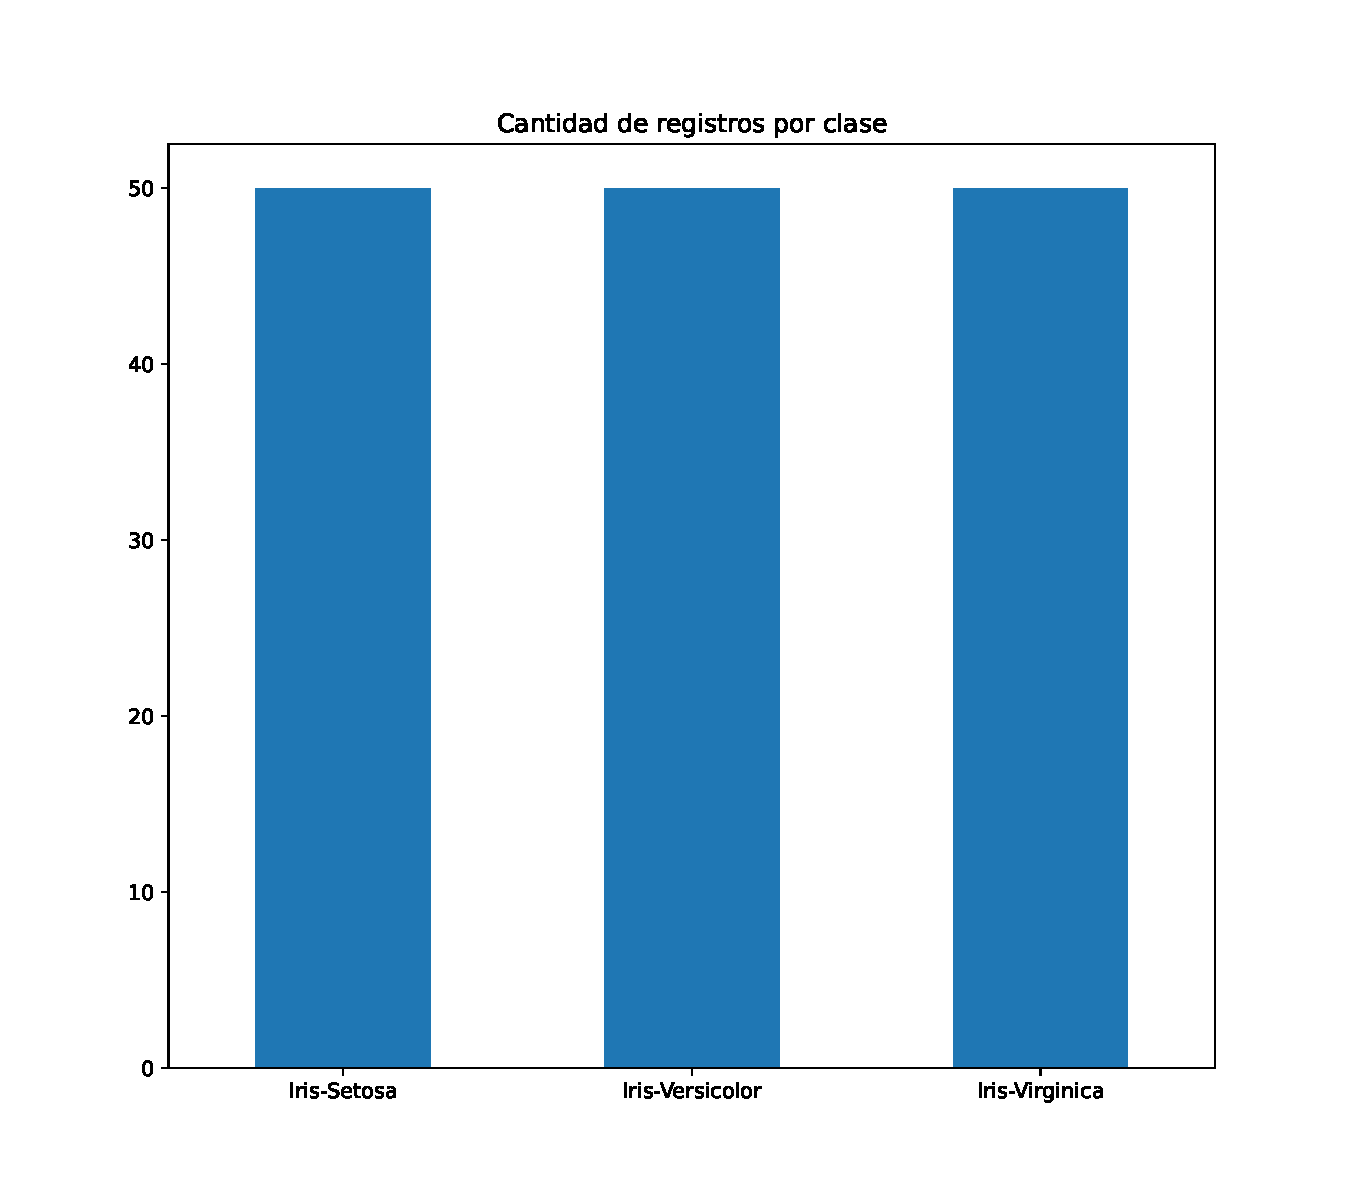
\includegraphics{/Users/pacaicedo/DataspellProjects/Atenea/Base/Consigna_files/figure-latex/unnamed-chunk-2-1.pdf}

\normalsize

Se advierte que en la columna Target:

\begin{itemize}
\tightlist
\item
  0 equivale a la especie Iris-Setosa,
\item
  1 a la especie Iris\_Versicolor
\item
  2 a la especie Iris-Virginica
\end{itemize}

\hypertarget{estaduxedstica-descriptiva-del-conjunto-de-datos}{%
\subsection{Estadística descriptiva del conjunto de
datos}\label{estaduxedstica-descriptiva-del-conjunto-de-datos}}

\begin{verbatim}
## -- Attaching packages --------------------------------------- tidyverse 1.3.1 --
\end{verbatim}

\begin{verbatim}
## v ggplot2 3.3.5     v purrr   0.3.4
## v tibble  3.1.5     v dplyr   1.0.7
## v tidyr   1.1.4     v stringr 1.4.0
## v readr   2.0.1     v forcats 0.5.1
\end{verbatim}

\begin{verbatim}
## -- Conflicts ------------------------------------------ tidyverse_conflicts() --
## x dplyr::filter() masks stats::filter()
## x dplyr::lag()    masks stats::lag()
\end{verbatim}

\begin{verbatim}
##   Sepal.Length    Sepal.Width     Petal.Length    Petal.Width   
##  Min.   :4.300   Min.   :2.000   Min.   :1.000   Min.   :0.100  
##  1st Qu.:5.100   1st Qu.:2.800   1st Qu.:1.600   1st Qu.:0.300  
##  Median :5.800   Median :3.000   Median :4.350   Median :1.300  
##  Mean   :5.843   Mean   :3.057   Mean   :3.758   Mean   :1.199  
##  3rd Qu.:6.400   3rd Qu.:3.300   3rd Qu.:5.100   3rd Qu.:1.800  
##  Max.   :7.900   Max.   :4.400   Max.   :6.900   Max.   :2.500  
##        Species  
##  setosa    :50  
##  versicolor:50  
##  virginica :50  
##                 
##                 
## 
\end{verbatim}

\hypertarget{tendencia-central}{%
\subsubsection{Tendencia central}\label{tendencia-central}}

\hypertarget{tendencia-central-para-la-especie-iris-setosa}{%
\paragraph{Tendencia central para la especie
Iris-Setosa}\label{tendencia-central-para-la-especie-iris-setosa}}

\hypertarget{tendencia-central-para-la-especie-iris-versicolor}{%
\paragraph{Tendencia central para la especie
Iris-Versicolor}\label{tendencia-central-para-la-especie-iris-versicolor}}

\hypertarget{tendencia-central-para-la-especie-iris-virginica}{%
\paragraph{Tendencia central para la especie
Iris-Virginica}\label{tendencia-central-para-la-especie-iris-virginica}}

\hypertarget{dispersiuxf3n}{%
\subsubsection{Dispersión}\label{dispersiuxf3n}}

\hypertarget{dispersiuxf3n-para-la-especie-iris-setosa}{%
\paragraph{Dispersión para la especie
Iris-Setosa}\label{dispersiuxf3n-para-la-especie-iris-setosa}}

\hypertarget{dispersiuxf3n-para-la-especie-iris-versicolor}{%
\paragraph{Dispersión para la especie
Iris-Versicolor}\label{dispersiuxf3n-para-la-especie-iris-versicolor}}

\hypertarget{dispersiuxf3n-para-la-especie-iris-virginica}{%
\paragraph{Dispersión para la especie
Iris-Virginica}\label{dispersiuxf3n-para-la-especie-iris-virginica}}

\end{document}
